%%=============================================================================
%% Methodologie
%%=============================================================================

\chapter{\IfLanguageName{dutch}{Methodologie}{Methodology}}
\label{ch:methodologie}

%% TODO: Hoe ben je te werk gegaan? Verdeel je onderzoek in grote fasen, en
%% licht in elke fase toe welke stappen je gevolgd hebt. Verantwoord waarom je
%% op deze manier te werk gegaan bent. Je moet kunnen aantonen dat je de best
%% mogelijke manier toegepast hebt om een antwoord te vinden op de
%% onderzoeksvraag.
\section{Scenario 1: alledaags gebruik}
\lipsum[1-4]

\section{Scenario 2: professioneel IT-gebruik}
\lipsum[1-4]

\section{Proof-of-concept Swift applicatie}
\begin{figure}[h]
    \centering
    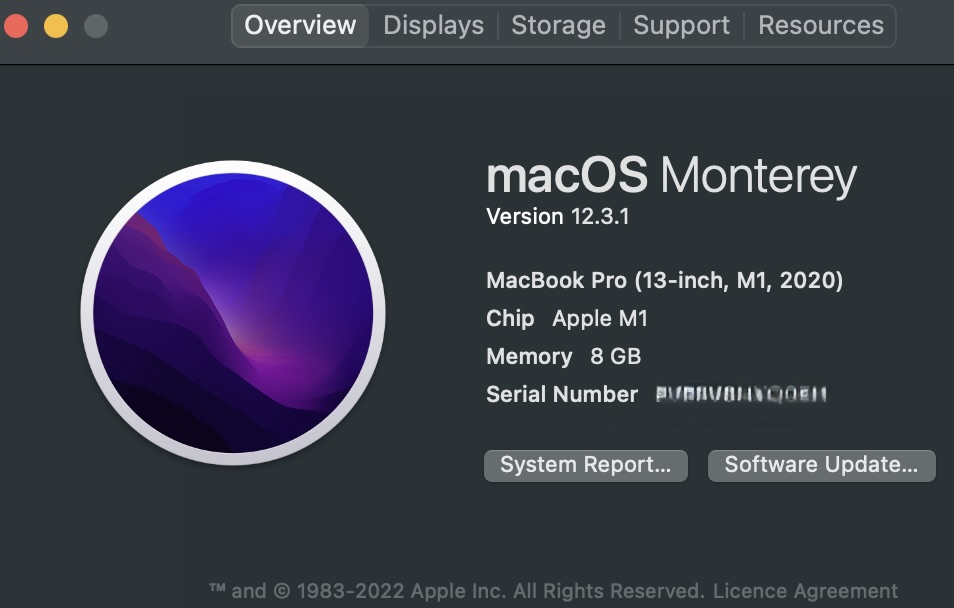
\includegraphics[width=100mm, scale=0.5]{img/overdezemac.jpeg}
    \caption{Het macOS 'Over deze Mac dialoogvenster'}
\end{figure}

\begin{figure}[h]
    \centering
    
\includegraphics[width=80mm, scale=0.7]{img/xcodeversie.jpeg}
    \caption{Het startscherm van Xcode 13}
\end{figure}

\begin{figure}[h]
    \centering
    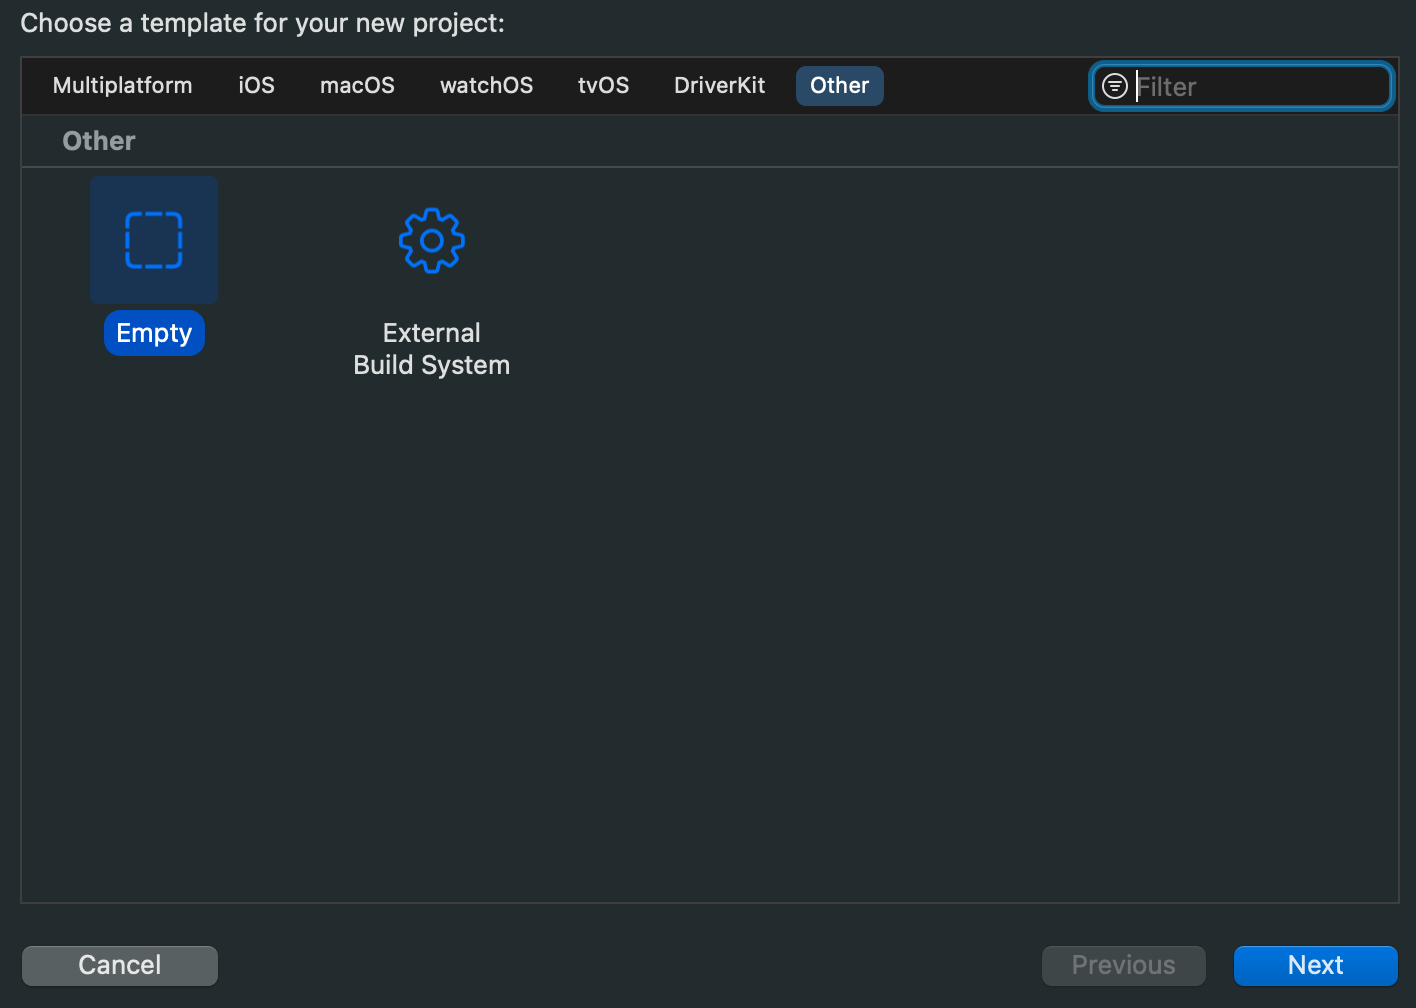
\includegraphics[width=\linewidth]{img/otherproject.png}
    \caption{Xcode 13 sjablonen}
\end{figure}

\begin{figure}[h]
    \centering
    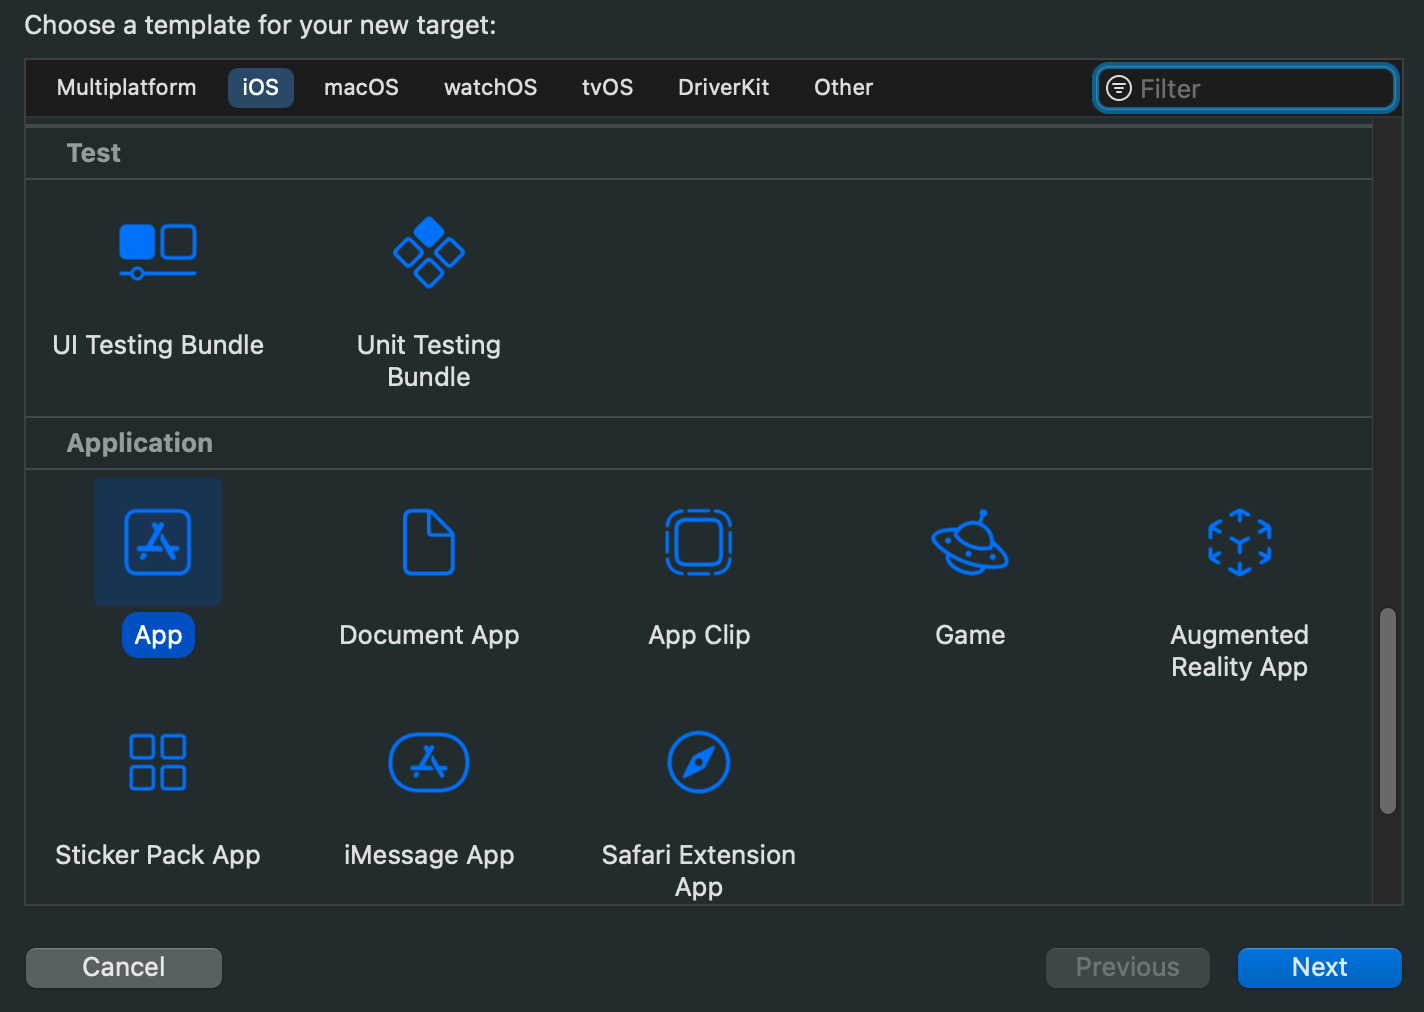
\includegraphics[width=\linewidth]{img/iostarget.png}
    \caption{Een overzicht van de verschillende targets}
\end{figure}

\begin{figure}[h]
    \centering
    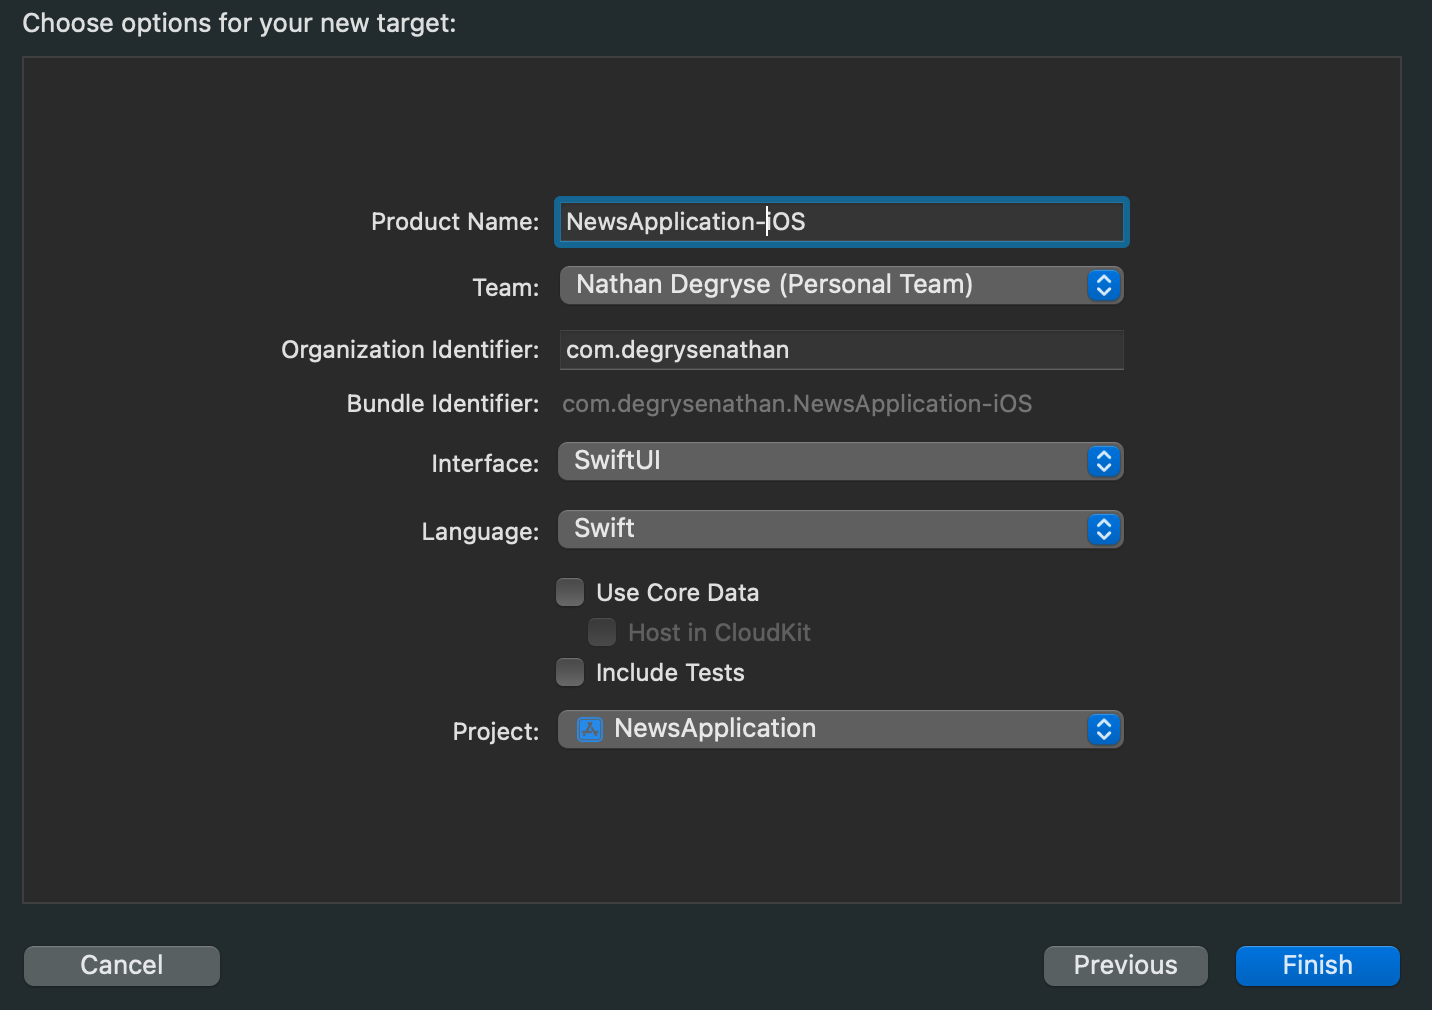
\includegraphics[width=\linewidth]{img/iostargetdetail.png}
    \caption{Een detailweergave van het iOS target}
\end{figure}

\begin{lstlisting}
    
    //  Article.swift
    //  NewsApplication-iOS
    //
    //  Created by Nathan Degryse on 11/05/2022.
    
    import Foundation
    
    enum Subject: String {
        case all = "All"
        case sport = "Sport"
        case internationaal = "Internationaal"
        case regionaal = "Regionaal"
        case politiek = "Politiek"
    }
    
    extension Subject {
        
        var title: String {
            switch self {
                case .all:
                return "All"
                case .sport:
                return "Sport"
                case .internationaal:
                return "Internationaal"
                case .regionaal:
                return "Regionaal"
                case .politiek:
                return "Politiek"
            }
        }
        
    }
    
    struct Article: Identifiable{
        let id = UUID()
        let name: String
        let photo: String
        let description: String
        let rating: Int?
        let subject: Subject
    }
    
\end{lstlisting}

\begin{figure}[h]
    \centering
    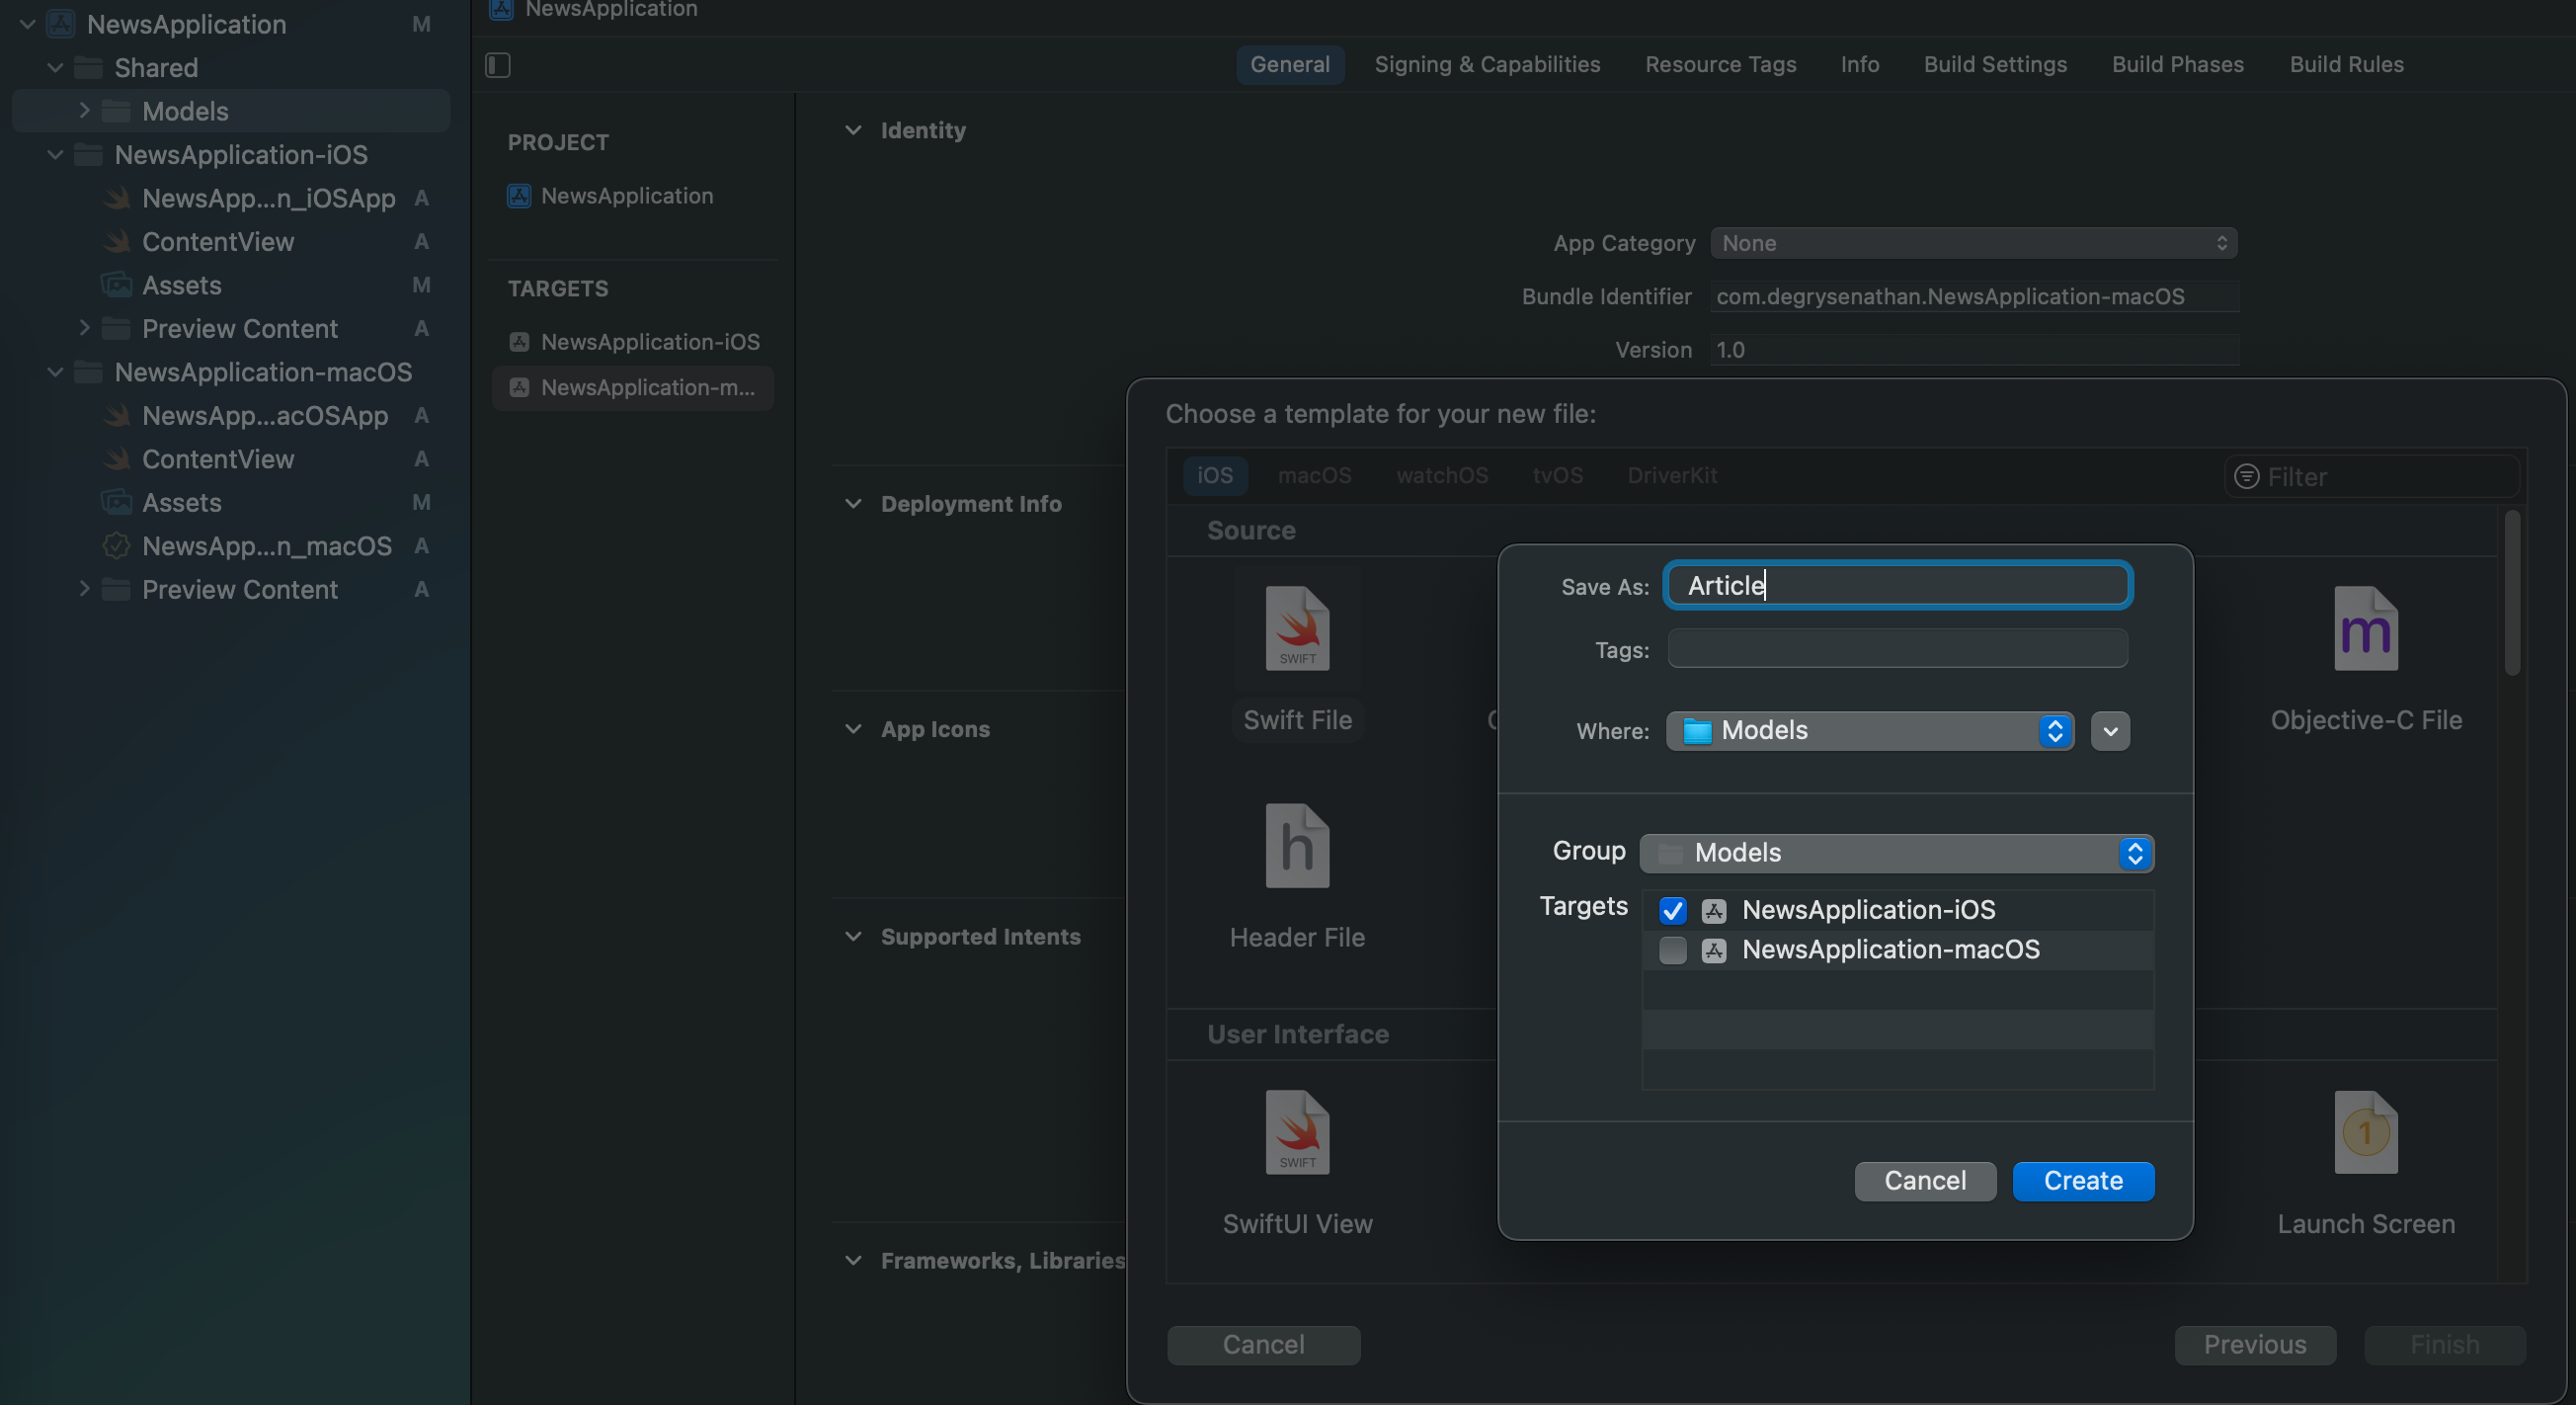
\includegraphics[width=\linewidth]{img/articleswift.png}
    \caption{Een overzicht van het initialisatievenster van Article.swift}
\end{figure}

\begin{figure}[h]
    \centering
    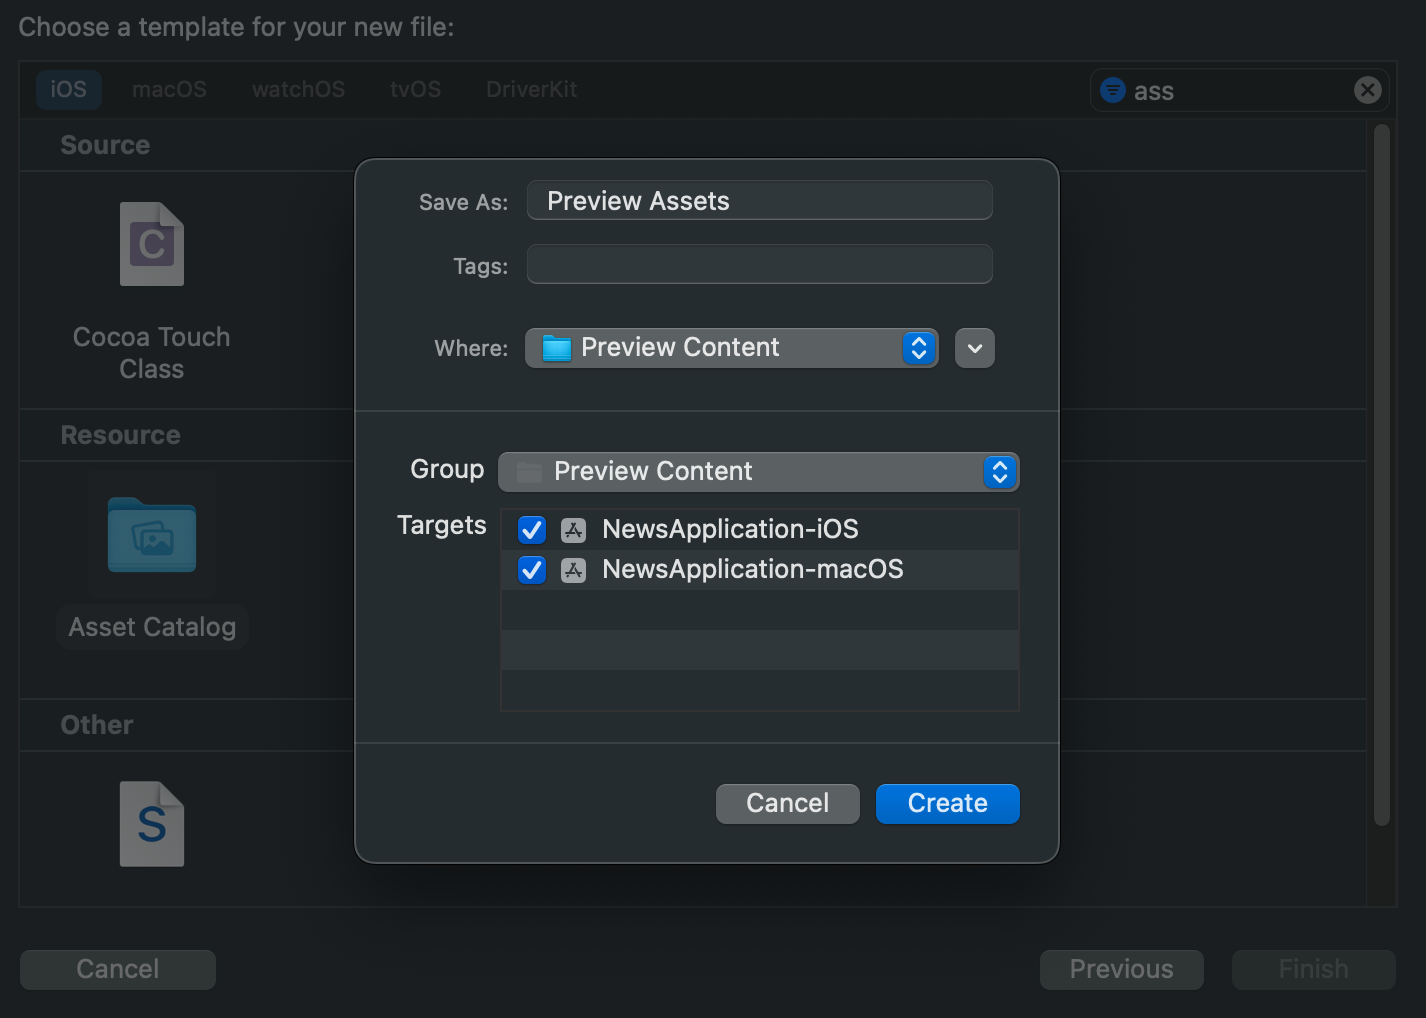
\includegraphics[width=\linewidth]{img/previewassets.png}
    \caption{Een overzicht van het initialisatievenster van de preview assets}
\end{figure}

\begin{figure}[h]
    \centering
    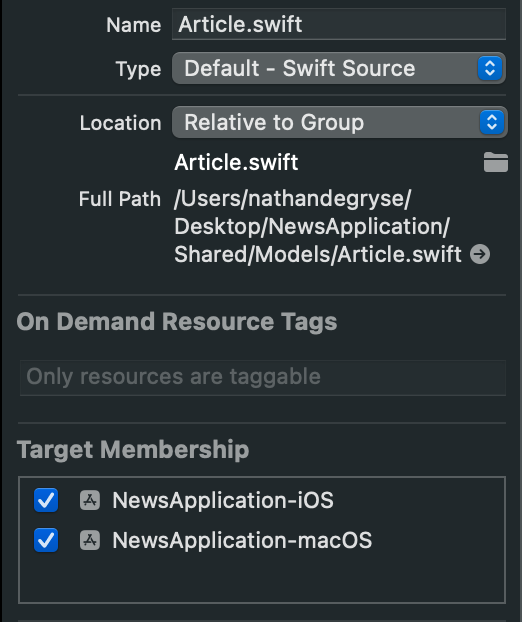
\includegraphics[width=80mm, scale=0.5]{img/articletargetmembership.png}
    \caption{Een overzicht van het targetmembership}
\end{figure}

\begin{figure}[h]
    \centering
    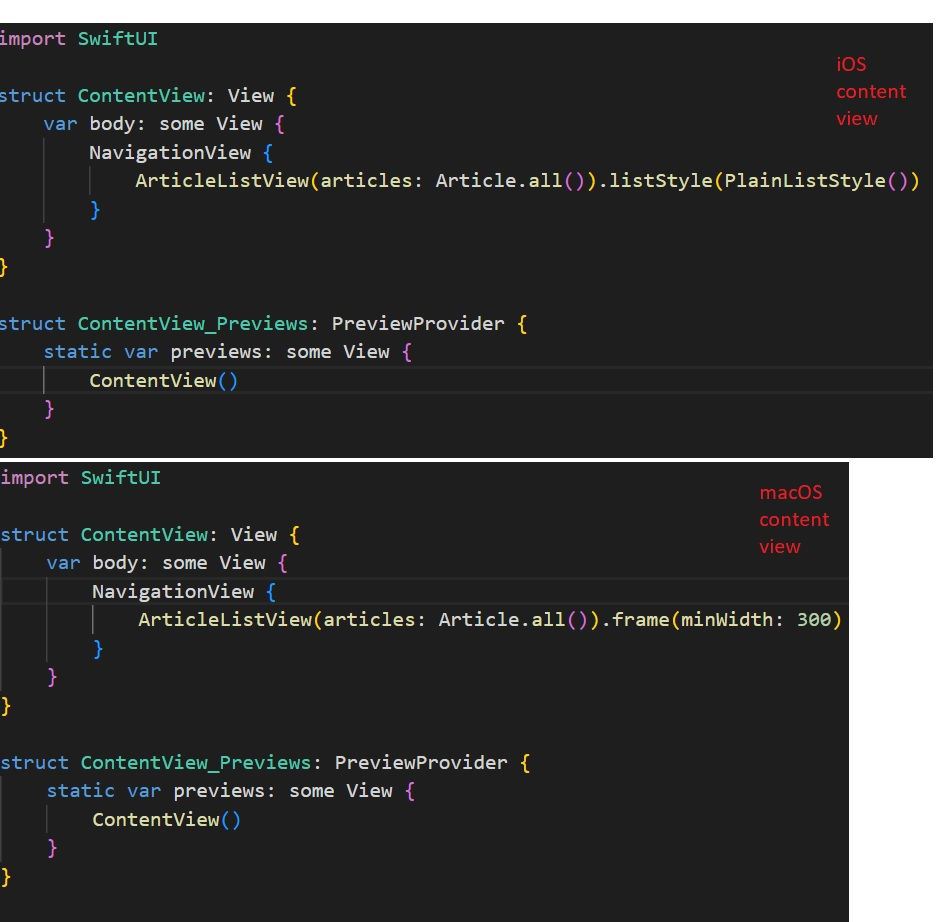
\includegraphics[width=\linewidth]{img/contentview.jpg}
    \caption{Een weergave van de ContentView files}
\end{figure}


\begin{figure}[h]
    \centering
    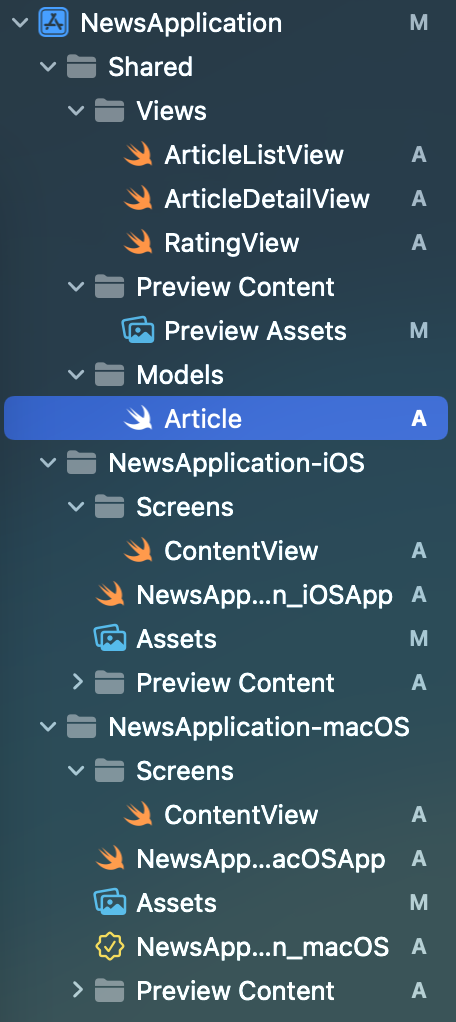
\includegraphics[width=50mm, scale=0.5]{img/applicatiestructuur.png}
    \caption{Een systematisch overzicht van de applicatiestructuur}
\end{figure}

\begin{figure}[h]
    \centering
    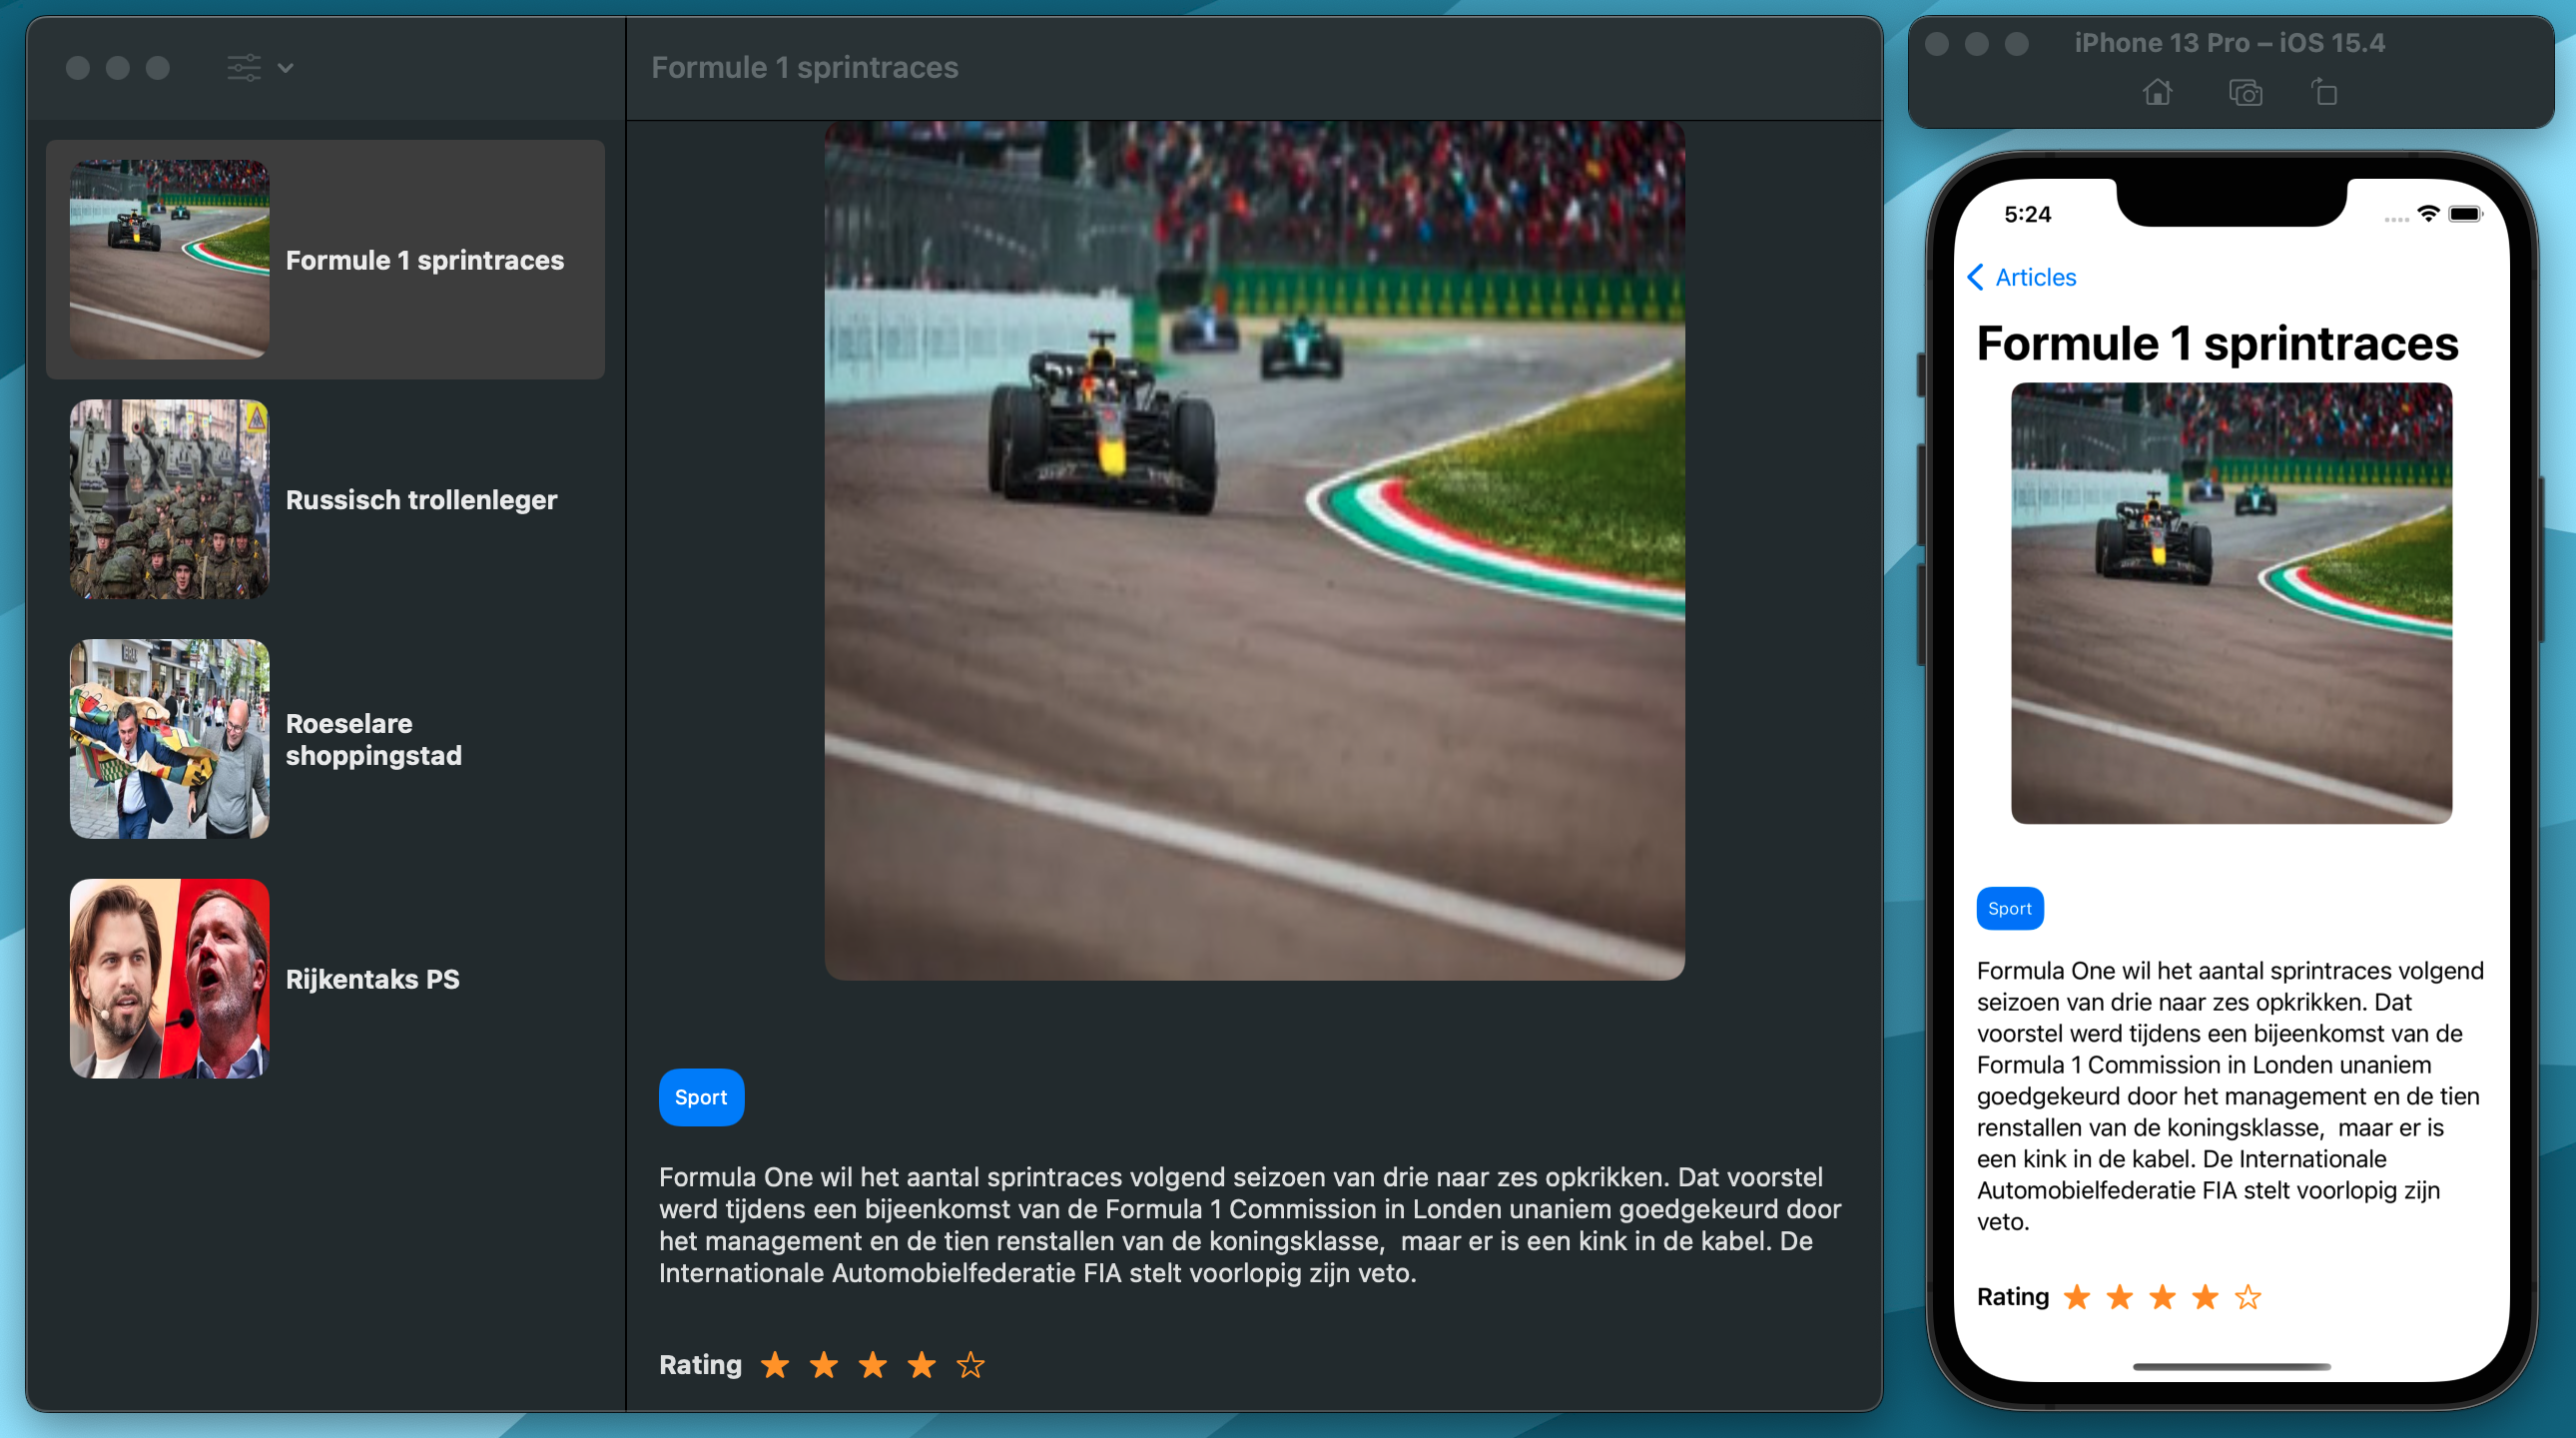
\includegraphics[width=\linewidth]{img/iosenmacosapplicatie.png}
    \caption{Een overzicht van de iOS en macOS nieuwsapplicatie}
\end{figure}
